\documentclass[a4paper,10pt]{ltjsarticle}
\usepackage{graphicx}
\usepackage{luatexja-fontspec}
\usepackage{caption}
\usepackage{amsmath,amssymb,bm,braket}
\usepackage[english]{babel}
\usepackage{multicol}
\usepackage{titlesec}
%\usepackage{gnuplot-lua-tikz}
\usepackage[top=20truemm,bottom=20truemm,left=20truemm,right=20truemm]{geometry}
\usepackage{array}
\usepackage{upgreek}
\usepackage{fancyhdr}
\renewcommand{\refname}{}
\usepackage{listings,jvlisting}
\usepackage{tikz}
\usepackage[thmmarks,amsmath]{ntheorem}
\usepackage[version=3]{mhchem}
\usetikzlibrary{external}
\tikzexternalize
\lstset{
  basicstyle={\ttfamily},
  identifierstyle={\small},
  commentstyle={\smallitshape},
  keywordstyle={\small\bfseries},
  ndkeywordstyle={\small},
  stringstyle={\small\ttfamily},
  frame={tb},
  breaklines=true,
  columns=[l]{fullflexible},
  numbers=left,
  xrightmargin=0pt,
  xleftmargin=3pt,
  numberstyle={\scriptsize},
  stepnumber=1,
  numbersep=1pt,
  lineskip=-0.5ex
}
\captionsetup[figure]{format=plain, labelformat=simple, labelsep=quad,labelfont=bf,name={Fig.}}
\captionsetup[table]{format=plain, labelformat=simple, labelsep=quad,labelfont=bf}
\parindent = 0pt
%[BoldFont=HGSMinchoE]{MSMincho}[BoldFont=HiraMinProN-W6]{HiraMinPro-W3}
\titleformat{\section}{\normalfont\fontsize{9}{10}\bfseries\fontspec{Times New Roman}}{\thesection.}{1em}{}
\usepackage[backend=biber,sorting=none,style=numeric,maxnames=99,minnames=1]{biblatex}
\addbibresource{utility/REFERENCES.bib}
\defbibheading{bibliography}[\refname]{%
  \section*{REFERENCES}%
  \vspace{-7pt}  % ここで空白を調整。お好みの値に変更してください。
}
\newfontfamily\subsectionfont{Times New Roman} % サブセクション用フォント
\titleformat{\subsection}
  {\normalfont\large\bfseries} % サブセクションのフォントを指定
  {\thesubsection}{1em}{}
\renewbibmacro{in:}{}
\renewbibmacro*{journal+issuetitle}{%
  \addcomma\space% カンマとスペースを追加
  \usebibmacro{journal}%
  \setunit*{\addspace}%
  \usebibmacro{volume+number+eid}%
  \setunit{\addspace}%
  \printfield{note}%
  \newunit
}
\renewbibmacro*{volume+number+eid}{
  \printfield{volume}%
  \setunit*{\addnbspace}%
  \printfield{number}%
  \setunit{\addcomma\space}%
  \printfield{eid}
}
\DeclareFieldFormat[article]{volume}{\textbf{#1}}
\DeclareFieldFormat[article]{pages}{#1}
\DeclareFieldFormat{journaltitle}{#1}
\usepackage{hyperref}
\renewenvironment{abstract}{\par\noindent}{\par}
%\pagenumbering{gobble}
\usepackage{docmute}
\usepackage{setspace}
\usepackage{titlesec} % 見出しのカスタマイズ用

% セクションのフォーマットをカスタマイズ
\titleformat{\section}
  {} % フォントサイズとスタイル
  {\Large\bfseries\thesection\ \ }               % 番号の前の内容(空白)
  {0em}            % 番号とタイトルの間の間隔
  {\Large\bfseries}


\theoremstyle{plain}
\theoremheaderfont{\normalfont\bfseries}
\theorembodyfont{\itshape}   % 本文を斜体に
\theoremseparator{.}         % タイトルと本文の区切りを「.」に設定
\newtheorem{definition}{Definition}
\begin{document}
\centerline{\LARGE\bfseries unfolding Color Codeの誤り耐性 その3}
\vspace{10pt}
 前回に引き続き、Color Codeのunfolding操作について、符号距離3のときの誤り耐性を調べてみた。今回はstimで符号距離3の場合を実装し、エラー伝播、測定エラーがあるような状況でも実効的な符号距離が3になっていることを確かめた。
\section{Unfolding過程のエラー検出}{
    \begin{figure}[h]
        \centering
        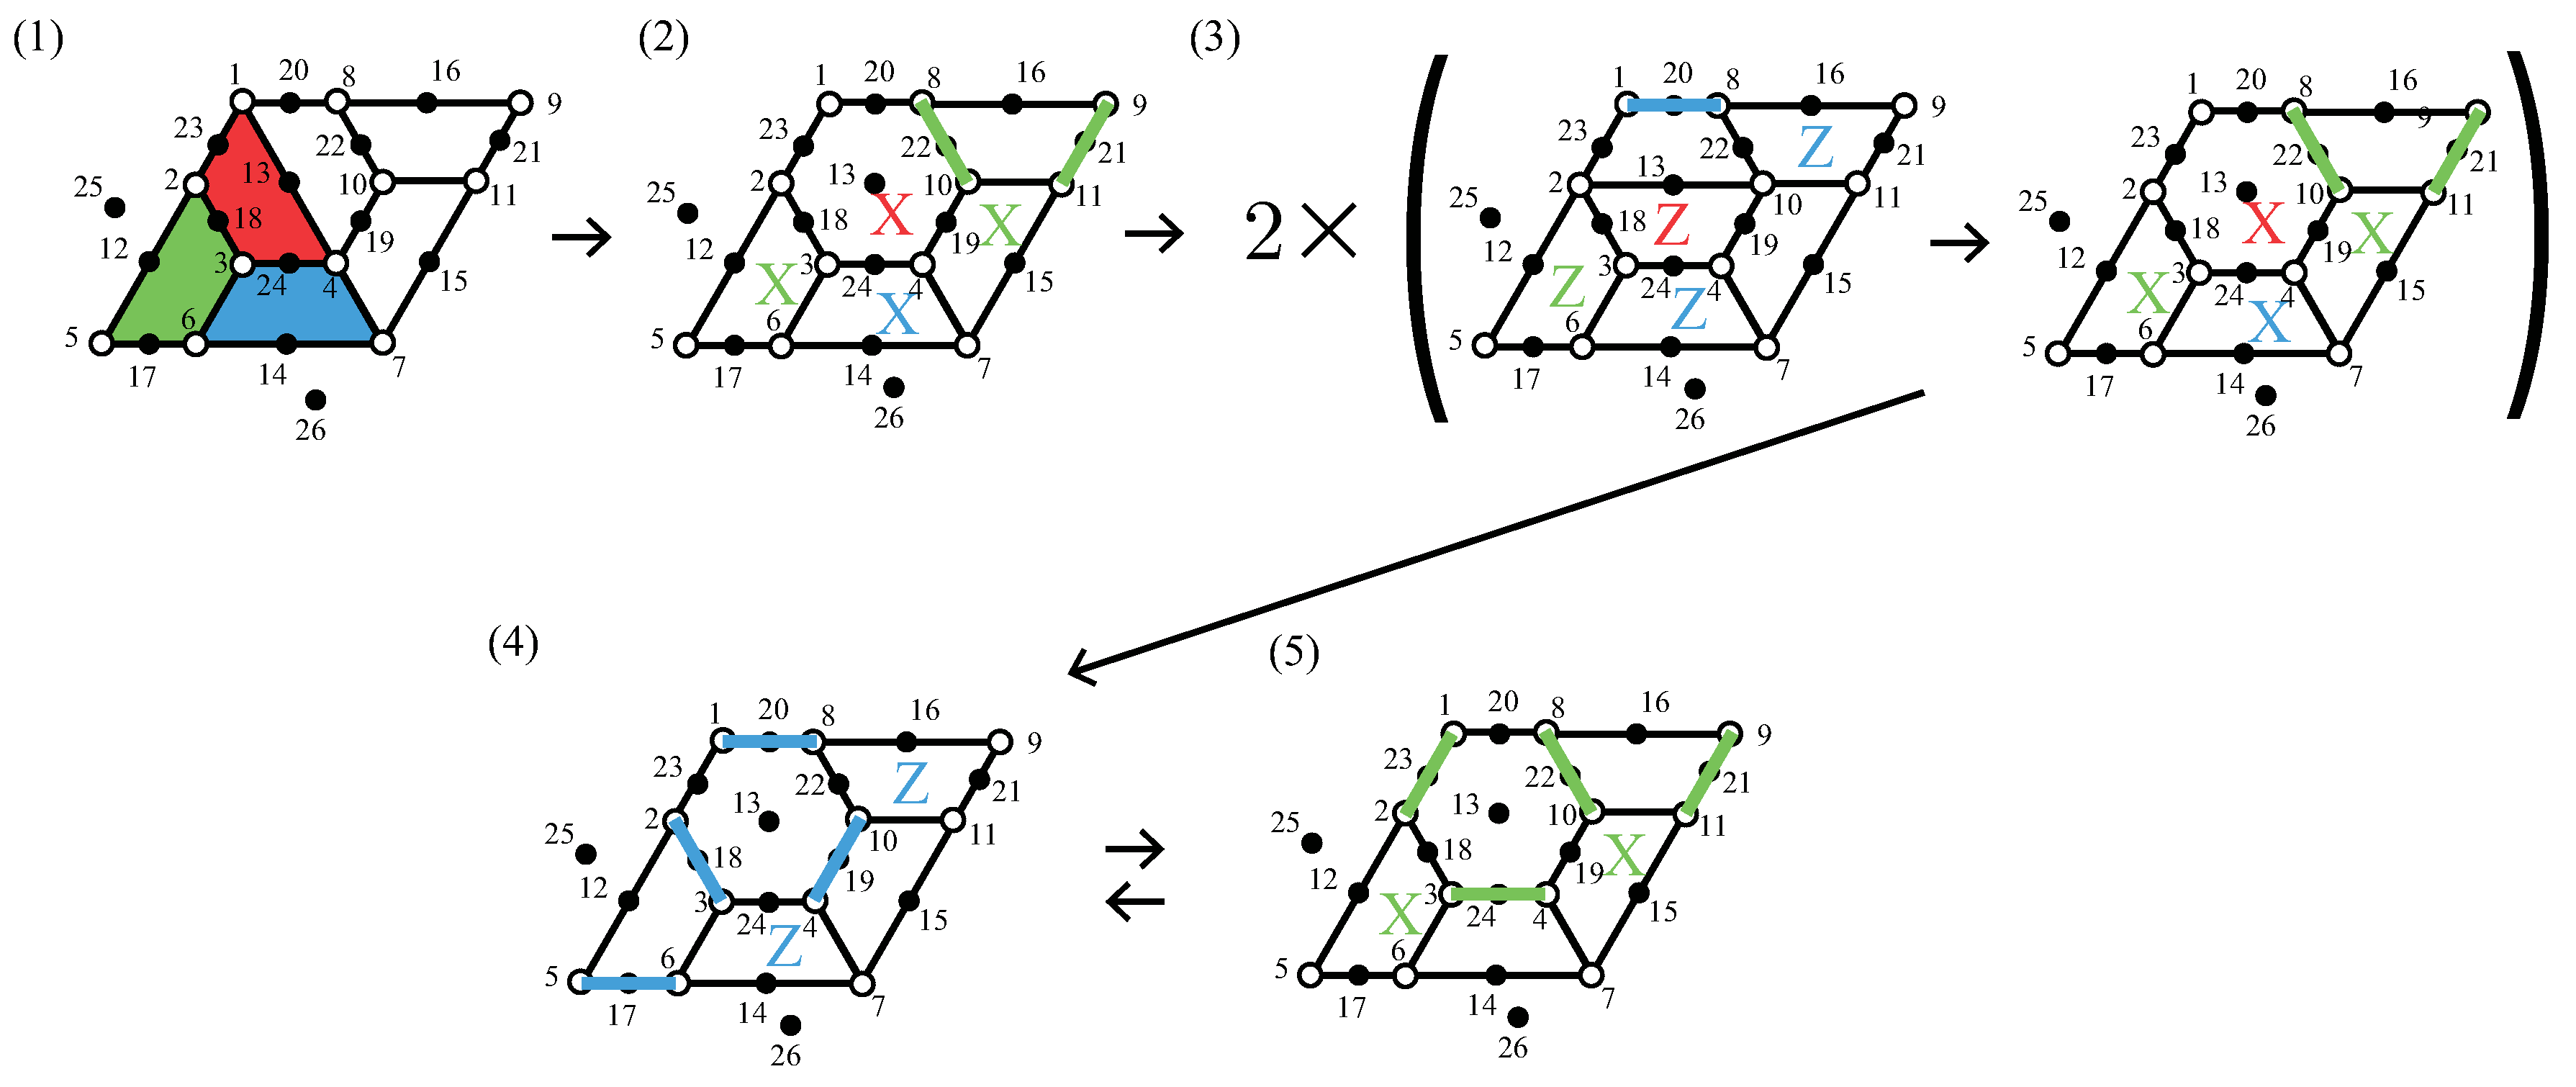
\includegraphics[scale=0.28]{figure/figure1.eps}
        \caption{ }
        \label{figure1}
    \end{figure}

     前回の資料(unfolding\_color\_code\_3.pdf)からの変更点をまず解説する。最終的なプロトコルをFig.\ref{figure1}に示す。白丸はdata qubit、黒丸12-24はその周りのdata qubitに対してシンドローム測定をする ancilla qubitであり、黒丸25,26はflag qubitである。(1)について、ここは前回と変わっていない、右上の部分にunfoldingするためのqubitを$\ket{0}$で用意する。qubit 25, 26は後のエラー検出のために欠かせないflag qubitである。(2),(3)は前回と大きく異なる。まず(2)から、前回はunfoldingの始めはZ stabilizerでシンドローム測定をしていたが、それをX stabilizerからに変更した。また、ancilla 12に関する4-weight X stabilizer測定についてはflag qubit を用いて2個のXエラーが伝播したかどうかをflag qubit 25を用いて監視しておく(要はシンドローム測定の2個目と3個目のCNOTの間でancilla 12にXエラーが起きたかどうかを監視)。Ancilla 14についても、同様にflag qubit 26を使って2個のXエラーが伝播したかどうかを監視しておく。次に(3)は前回とは異なる形のZ stabilizer 測定を行うようにし、変換途中のZ stabilizerとX Stabilizer測定を2回繰り返すように設計されている(ここでは、2回繰り返すと書いているが、本質的には(2)の形のX stabilizer 測定を符号距離回だけ行うことがエラー検出するうえで必要だということ。詳細は後で説明。)。また、Z stabilizer測定ではancilla 12について2個のZエラーが伝播したかどうかを監視、X stabilizer測定は(2)と全く同じ。(4)(5)は前回と同じ。\\
     それでは、(2)の形のX stabilizer 測定を符号距離回だけ行わなければならない理由を説明する。それは、ancilla 14を使う青色X stabilizerを捨てるからである。具体的に説明すると、例えば、(2)のシンドローム測定のCNOTで2 qubit depolarizing errorがancilla 14とdata qubit 7に確率$p$で発生したとすると、そのエラーの種類が確率$1/15$でancilla 14にZゲート、data qubit 7にZゲートだった場合、そのようなエラーが起きる確率は$p/15$である。また、このエラーは(2)のシンドローム値を反転させない、かつred boundaryに存在するX logical operatorと反可換である。そのため、このエラーを検出するためにもう一回青色X stabilizerのシンドローム値を得ないといけない(これは、(3)の1回目のX stabilizer測定に対応)。しかし、またここでancilla 14にmeasurement errorが確率$p$で発生したとすると、(2)で発生したエラーはまだ検出できない。また、ここまでのエラーは確率$p^2/15$で起きるので、符号距離3を担保するためにはもう一回青色X stabilizerのシンドローム値を得ないといけない(これは、(3)の2回目のX stabilizer測定に対応)。この3回目の測定でもmeasurement errorが発生する確率は$p^3/15$であるので、これは検出できなくて良い($p^3/15$が起きる確率はdata qubit 1,2,5にエラーが起きる確率$p^3$より小さい)。ということで、$p^{d-1}$までの確率で起こるエラーを検出するためには$d$回同じことをしないといけない。\\
     次にflag qubitを用いる理由について説明する。例えば(2)のancilla 12に注目すると、これを用いるシンドローム測定によって伝搬する2つのXエラーは、(i)CNOTをqubit 2,3,5,6の順番でかければ、5,6に伝播、(ii)CNOTをqubit 3,6,2,5の順番でかければ、2,5に伝播する(ここでは、stabilizerを法として合同なものは無視)。(i)が起き、data qubit 7エラーが起きると、実効的な符号距離は2、(ii)が起き、data qubit 1にXエラーが起きると実効的な符号距離は2なので、どの順番でCNOTをかけても実効的な符号距離が2になってしまう。そのため、flag qubitで2つのXエラーの伝播を監視する必要がある。他のflag qubitも同じ。flag qubit を用いないweightが4以上のstabilizerについてはCNOTをかける順番が厳密に決まっている。4-weightは前回紹介した通り、6-weight(今回は赤X stabilizer)は例えばqubit 2,8,1,3,4,10の順番である。これは総当たりで調べた。
}

\section{検証}{
     検証はgoogleの\cite{lacroix2024}のappendix Cの2に載っていたMaxSATを解く形で行った(中身は全く理解していない)。この検証で、Zメモリ、Xメモリの実効的な符号距離がどちらも3になった。ただし、検証はColor Codeのシンドローム測定でエラーが起こらないという仮定で行った。
}

\printbibliography
\end{document}